\documentclass[11pt]{article}

\usepackage{graphicx}
\usepackage[margin=1in]{geometry}

\title{CS 513 Theory \& Practice of Data Cleaning\\[0.4em]
       \large Phase-I Report\\[0.2em]
       \normalsize Team ID: [Team-ID] $\mid$ [Optional Team Name]}
\author{[Name 1] \texttt{netid1@illinois.edu} \and
        [Name 2] \texttt{netid2@illinois.edu}}
\date{May 24, 2026}

\begin{document}

\maketitle

\begin{abstract}
This Phase-I report describes the NYPL historic menus dataset, defines three use cases,
identifies observable data quality problems, and outlines the data cleaning plan for Phase-II.
\end{abstract}

% ─────────────────────────────────────────────
\section{Description of Dataset}  % 25 pts

\subsection{Conceptual Model / Database Schema}  % 10 pts

The database schema is documented by the ER diagram below:

\begin{figure}[htbp]
    \centering
    
\includegraphics[width=\textwidth]{er_diagram.png}
    \caption{Entity-Relationship Diagram for the Restaurant Menu Dataset.}
    \label{fig:er_diagram}
\end{figure}

\subsection{Narrative Description}  % 15 pts

Some text.

% ─────────────────────────────────────────────
\section{Use Cases}  % 30 pts

\subsection{Target Use Case U1 --- Data Cleaning Necessary and Sufficient}  % 20 pts

What are the most popular dishes by decade, and how did their prices change over time?

\subsection{Zero Data Cleaning Use Case U0 --- Data Cleaning Not Necessary}  % 5 pts

How many menu pages does each menu have?

\subsection{Never Enough Use Case U2 --- Data Cleaning Not Sufficient}  % 5 pts

Which dishes were most enjoyed or preferred by diners?

% ─────────────────────────────────────────────
\section{Data Quality Problems}  % 30 pts

\subsection{Obvious Data Quality Problems with Evidence}  % 20 pts

\subsubsection*{Missing Data in Menu.csv}
Additionally, there are numerous missing values in the dataset. Specifically, in the \texttt{Menu.csv} file, there are attributes that, although present in the schema, have absolutely no data in the actual dataset. Furthermore, other valuable attributes like name, venue, place, and event have many empty entries as well (see Figure \ref{fig:missing_data}).

\begin{figure}[htbp]
    \centering
    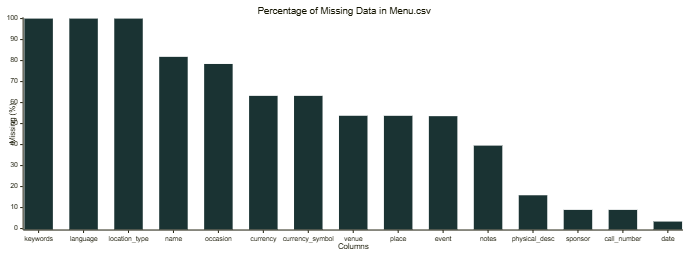
\includegraphics[width=\textwidth]{missing_data_chart.png}
    \caption{Missing Data Percentages in Menu.csv}
    \label{fig:missing_data}
\end{figure}

\subsubsection*{Data Inconsistencies and Formatting Variances}
The dataset has many spelling variations for what would appear to be the same concept. For example, using different roots of the word ``anniversary'' (including aniv, anniv, anniversary, anniversaryersary, annual), there are a variety of matching entries in the dataset.

Examples of this inconsistency for the root concept of ``anniversary'':
\begin{itemize}
    \item Root \textbf{`aniv'} $\rightarrow$ Appears as: \texttt{['ANIV;', '[ANIV?];']}
    \item Root \textbf{`anniv'} $\rightarrow$ Appears as: \texttt{['[ANNIV?];', '[?ANNIV?];', '(ANNIV);', '(ANNIV?);', '[ANNIV?]']}
    \item Root \textbf{`anniversary'} $\rightarrow$ Appears as: \texttt{['ANNIVERSARY;', 'ANNIVERSARY(?);', 'ANNIVERSARY', 'ANNIVERSARY (?);', 'ANNIVERSARY.', 'ANNIVERSARY?']}
    \item Root \textbf{`anniversaryersary'} $\rightarrow$ Appears as: \texttt{['ANNIVERSARYERSARY', 'ANNIVERSARYERSARY;']}
    \item Root \textbf{`annual'} $\rightarrow$ Appears as: \texttt{['ANNUAL', '[ANNUAL]', 'ANNUAL;']}
\end{itemize}

\subsubsection*{Data Type Variation}
There is also distinct data type variation. For example, in the \texttt{Dish} table's \texttt{name} column, there are 47 times where the name is purely numeric, while the remaining 423,204 names are all alphabetic. Although the name truly could be "15", this causes some ambiguity regarding what is actually meant by the name.

\subsection{Why Data Cleaning is Necessary for U1}  % 10 pts

Some text.

% ─────────────────────────────────────────────
\section{Initial Plan for Phase-II}  % 15 pts

\begin{description}
    \item[S1] \textbf{Dataset and use case review.} Some text.
    \item[S2] \textbf{Profiling D to identify DQ problems.} Some text.
    \item[S3] \textbf{Data cleaning proper.} Some text.
    \item[S4] \textbf{Data quality checking.} Some text.
    \item[S5] \textbf{Documenting and quantifying change.} Some text.
\end{description}

\end{document}